\chapter{Experiment Description }

The Compact Muon Solenoid (CMS) detector is a multi-purpose apparatus that operates at the LHC at CERN. Its name comes from the fact that is quite compact for all the detector material it contains ( 15 meters high and 21 meters long), it is designed to detect muons very accurately, and it has it has the most powerful solenoid magnet ever made. Along with ATLAS, is one of the two high luminosity experiments at CERN. In this chaper the components of the CMS are described. The silicon pixel tracker is described with more detail due the purposes of this thesis. 

\section{The Compact Muon Solenoid}

The Compact Muon Solenoid (CMS) experiment is one of four detectors placed  around the LHC. The CMS detector consist of several detection layers, having a total length of 21.6 m with a diameter of 14.6 m. It consist of a silicon tracker to provide a measurement of the trajectories of charged particles, a 3.8 Tesla superconducting solenoid, an electronic and hadronic calorimeter to meausure particle energy, and a muon detection system \cite{CMS_Exp_2008}. A diagram of a perspective view of the CMS detector is shown in Fig. \ref{detector_CMS}.\\
%%%%%%%%%%%% PARAGRAPH TO SUMMARY THE LAST 3 SECTION (ECAL, HCAL AND MUONS SYSTEM)%%%%%%
%%%%%%%%%%%%%%%%%%%%%%%%%%%%%%%%%%%%%%%%%%%%%%%%%%%%%%%%%%%%%%%%%%%%%%%%%%%%%%%%%%%%%%%%%
The electromagnetic calorimeter of CMS (ECAL) is a hermetic homogeneous calorimeter made of 61 200 lead tungstate (PbWO4) crystals mounted in the central barrel part, closed by 7 324 crystals in each of the two endcaps. A preshower detector is placed in front of the endcap crystals. Avalanche photodiodes (APDs) are used as photodetectors in the barrel and vacuum phototriodes (VPTs) in the endcaps \cite{CMS_Exp_2008}.\\
The ECAL is surrounded by a brass/scintillator sampling hadron calorimeter (HCAL). The scintillation light is converted by wavelength-shifting (WLS) fibres embedded in the scintillator tiles and channeled to photodetectors via clear fibres. This light is detected by photodetectors (hybrid photodiodes, or HPDs) that can provide gain and operate in high axial magnetic fields. The Cerenkov light emitted in the quartz fibres is detected by photomultipliers \cite{CMS_Exp_2008}.\\ 
After the HCAL and the 13-m-long, 6-m-inner-diameter, 4-T superconducting solenoid, the muon detector system is placed. CMS uses 3 types of gaseous particle detectors for muon identification. Due to the shape of the solenoid magnet, the muon system was naturally driven to have a cylindrical, barrel section and 2 planar endcap regions \cite{CMS_Exp_2008}.\\
The tracker system is described with detail in the next section.\\
%%%%%%%%%%%%%%%%%%%%%%%%%%%%%%%%%%%%%%%%%%%%%%%%%%%%%%%%%%%%%%%%%%%%%%%%%%%%%%%%%%%%%%%5
A sketch of a transverse slice of the CMS detector, with specific particle interactions, is shown in Fig. \ref{slice_CMS}. A simplified summary of particle interaction (and detection) is described as follows. Starting from the beam interaction region, particles first enter a tracker, in which charged-particle trajectories (tracks) and origins (vertices) are reconstructed from signals (hits) in the sensitive layers. The tracker is immersed in a magnetic field that bends the trajectories and allows the electric charges and momenta of charged particles to be measured. Electrons and photons are then absorbed in an electromagnetic calorimeter (ECAL). The corresponding electromagnetic showers are detected as clusters of energy recorded in neighbouring cells, from which the energy and direction of the particles can be determined. Charged and neutral hadrons may initiate a hadronic shower in the ECAL as well, which is subsequently absorbed in the hadron calorimeter (HCAL). Muons and neutrinos traverse the calorimeters with little or no interactions. While neutrinos escape undetected, muons produce hits in additional tracking layers called muon system, located outside the calorimeters \cite{det_summary}.\\
\begin{center}
  \begin{figure}[ht]
    \centering
    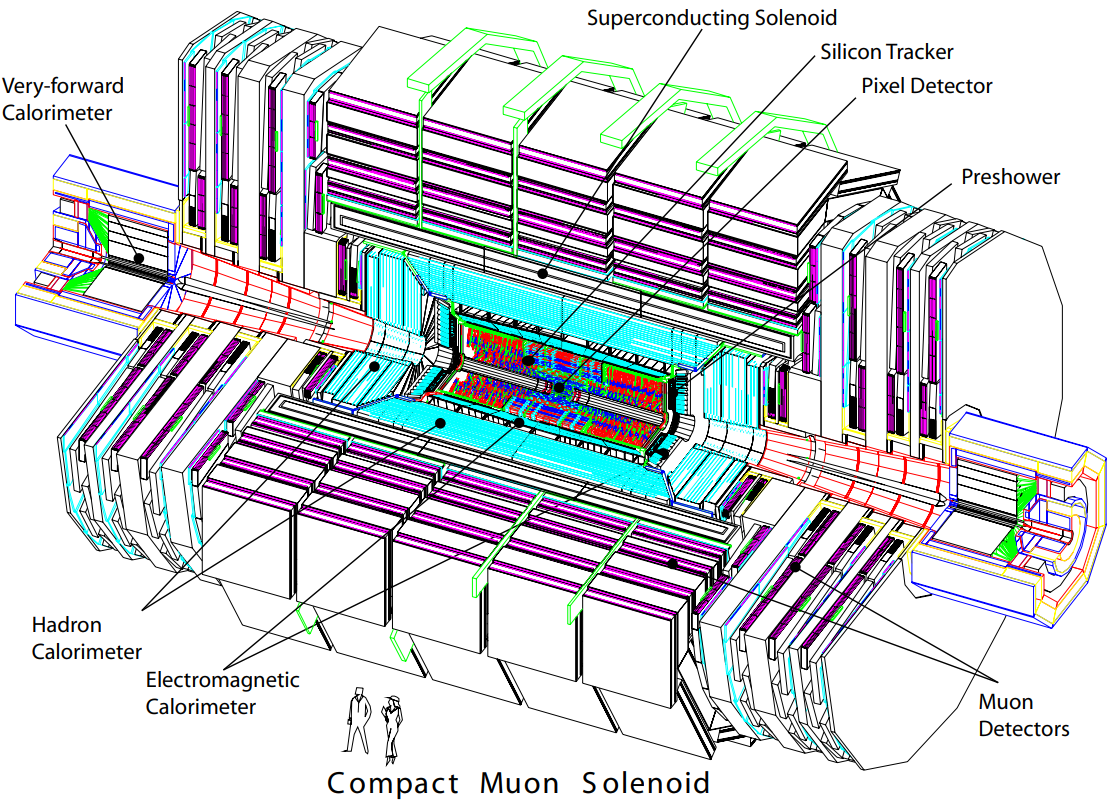
\includegraphics[scale=.3]{Chapter2/CMS_detector_simple.png}
    \caption[Perspective view of the CMS detector]{Perspective view of the CMS detector.}
    \label{detector_CMS}
  \end{figure}
\end{center}

\begin{center}
  \begin{figure}[ht]
    \centering
    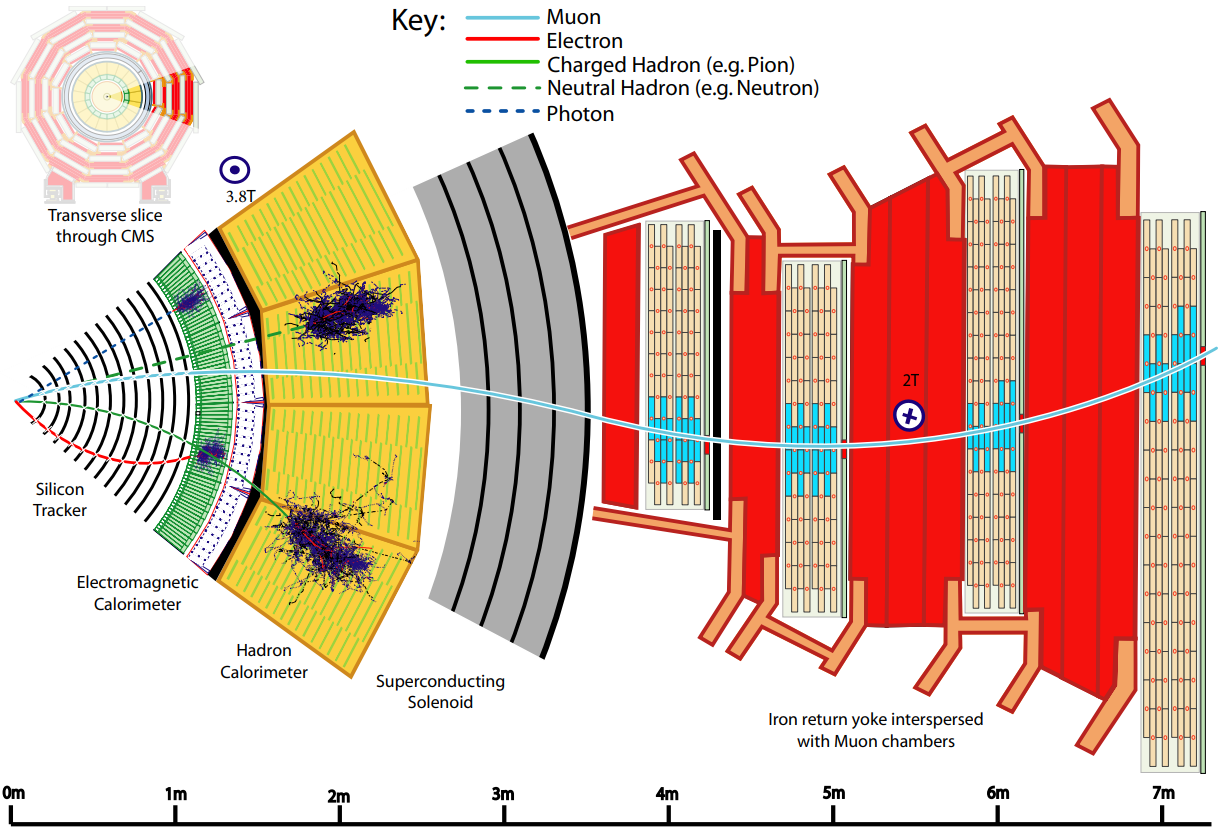
\includegraphics[scale=.3]{Chapter2/slice_det.png}
    \caption[Transverse slice fo CMS detector]{Sketch of a transverse slice of the CMS detector with specific particle interactions, from the beam interaction region to the muon detector. The muon and the charged pion are positively charged, and the electron is negatively charged \cite{det_summary}.}
    \label{slice_CMS}
  \end{figure}
\end{center}


The coordinate system adopted by CMS has the origin at the center of the detector, the $y$-axis pointing vertically upward, and the $x$-axis pointing radially inward toward the center of the LHC. Thus, the z-axis points along the beam direction toward the Jura mountains from LHC Point 5. The azimuthal angle $\varphi$ is measured from the $x$-axis in the $x-y$ plane and the radial coordinate in this plane is denoted by $r$. The polar angle $\theta$ is measured from the $z$-axis. Pseudorapidity is defined as $\eta=- \ln \tan (\theta/2)$ \cite{CMS_Exp_2008}.\\
%The components of the CMS detector, the tracking system, electromagnetic and hadronic calorimeter, and the muon system, are discribed briefly in the following subsections.

\section{CMS Tracking System}
The measurement of the momenta of charged particles is an essential aspect of any large particle physics experiment. Regardless of the medium through which a charged particle travels, it leaves a trail of ionised atoms and liberated electrons. By detecting this ionisation it is possible to reconstruct the trajectory of a charged particle. A charged particle will leave a hit in a silicon sensor in each cylindrical layer from which the trajectory of the charged particle track can be reconstructed.\cite{thomson_2013}.\\
When a charged particle passes through a medium, it interacts electromagnetically with the atomic electrons and loses energy through the ionisation of the atoms \cite{thomson_2013}. The theory of such losses, which are due dominantly to Coulomb scattering from the atomic electrons, was worked out by Bethe, Bloch and others in the 1930s. The result is called the Bethe–Bloch formula: \cite{Martin2017_book}:

\begin{equation}
  -\frac{dE}{dx}= \frac{Dq^{2}n_{e}}{\beta ^{2}} \biggl[ \ln \left(\frac{2m_{e}c^{2}\gamma^{2}}{I} \right) -\beta^{2} -\frac{\delta(\gamma)}{2}  \biggr]
  \label{bethe}
\end{equation}

$x$ is the distance travelled through the medium, $m_{e}$ is the electron mass, $\beta=v/c$,  $\gamma =(1-\beta^{2})^{-1/2}$ and $D=\frac{4\pi \alpha^{2} \hslash^{2}}{m_{e}}=$5.1$\times 10^{-25}$MeV cm$^{2}$. The other constants refers to the medium: $n_{e}$ is the electron density, $I$ is the mean ionisation potencial of the atoms averaged over all electrons (given approximately by $I$=10$Z$eV for $Z>$20) and $\delta$ is a dielectric screening correction that is only important for highly relativistic particles. %The corresponding formula for spin–1/2 particles differs from this, but in practice the differences are small and may be neglected for the discussion of the main features of ionisation energy losses. It is common practice to divide eq. \ref{bethe} by the mass density $\rho$ and to redefine $x$ as the density multiplied by the distance travelled, so that $\frac{dE}{dx}\rightarrow -\frac{1}{\rho}\frac{dE}{dx}$, beeing $x$ now measured in g/cm$^{2}$. As can be seen in \ref{bethe}, $-dE/dx$ falls rapidly as the velocity increases from zero because of the $1/\beta$ factor. All particles have a region of ‘minimum ionisation’ for $\beta \gamma$ \cite{Martin2017_book}.\\

The tracking detector in the CMS experiment is based on semiconductor technology using silicon pixels and strips. It is composed of two sub systems, the pixel tracker (the closest to the interaction vertex) and the  strip tracker \cite{CMS_Exp_2008}. The Pixel detector is described below. 

\subsection{Pixel Detector and Clustering}
\label{pixel_clust_reco}
The pixel tracker originally consisted of three barrel layers at radii of 44, 73, and 102 mm and two endcap disks on each end \cite{CMS_Exp_2008}. With the upgrade of the accelerators during the first long shutdown (LS1, 2013-2014) the original pixel detector has been replaced by a new system referred to as the CMS Phase-1 pixel detector. The installation of the CMS Phase-1 pixel detector took place during the extended year-end technical stop of the LHC in 2016/2017. The layout of the CMS Phase-1 pixel detector is optimized to have four-hit coverage over the pseudorapidity range ($|\eta|<2.5$), improved pattern recognition and track reconstruction, and added redundancy to cope with hit losses \cite{phase1_Pixel_Detector}. \\
The CMS Phase-1 pixel detector consists of four concentric barrel layers (L1-L4) at radii of 29, 68, 109, and 160 mm, and three disks (D1-D3) on each end at distances of 291, 396, and 516 mm from the center of the detector. The layout of the CMS Phase-1 pixel detector is shown  in Fig. \ref{phase1_pixel_detector}. The total silicon area of the CMS Phase-1 pixel detector is 1.9 $\text{m}^{2}$, while the total silicon area of the original pixel detector was 1.1 $\text{m}^{2}$.

\begin{center}
  \begin{figure}[ht]
    \centering
    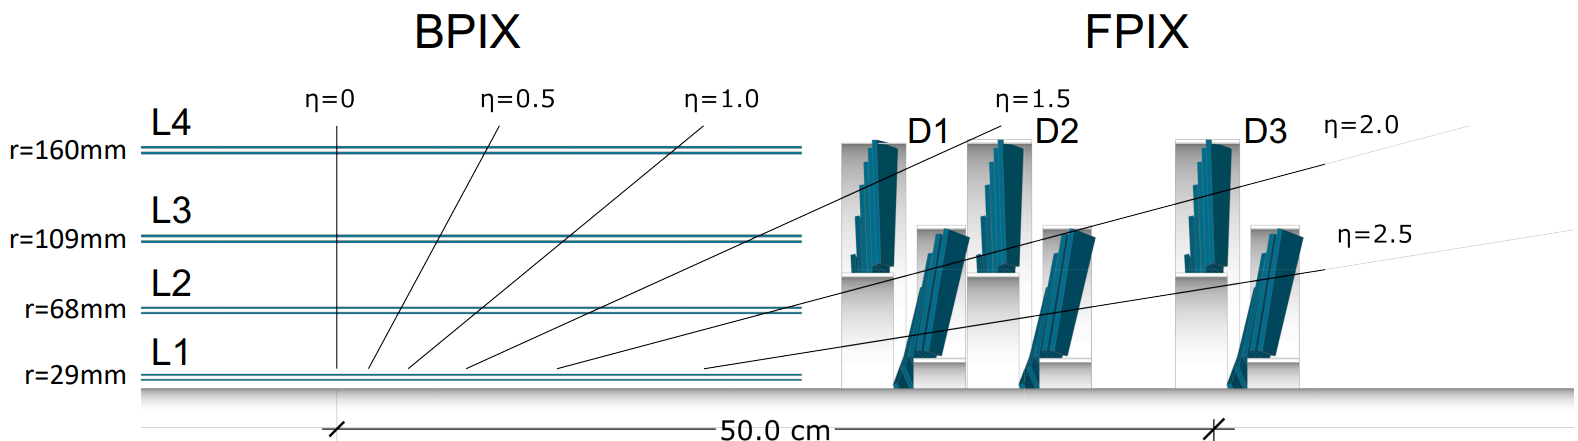
\includegraphics[scale=.26]{Chapter2/phase1_PixelDetector.png}
    \caption[CMS Phase-1 pixel detector]{Layout of the CMS Phase-1 pixel detector in longitudinal view\cite{phase1_Pixel_Detector}.}
    \label{phase1_pixel_detector}
  \end{figure}
\end{center}


The CMS Phase-1 pixel detector is built from 1856 segmented silicon sensor modules, where 1184 modules are used in the barrel pixel detector (BPIX) and 672 modules are used for the forward disks (FPIX). Each module consists of a sensor with 160$\times$416 pixels connected to 16 readout chips (ROCs). In total there are 124 million readout channels \cite{phase1_Pixel_Detector}.\\
The CMS Phase-1 pixel detector uses a similar module design as the BPIX modules of the original detector. A pixel detector module is built from a planar silicon sensor with a size of 18.6 $\times$ 66.6 $\text{mm}^{2}$ (active area of 16.2 $\times$ 64.8 $\text{mm}^{2}$), bump-bonded to an array of 2$\times$8 ROCs. Each ROC is segmented into 4160 readout channels and reads out the pulse height information for each pixel. The standard pixel size is 100$\times$150 $\mu m^{2}$, as in the original pixel detector.% Since two ROCs can only be placed at some minimum distance from each other, pixels along the ROC boundaries have twice the area and those at the corners have four times the area of a standard pixel. In order to simplify module production and maintenance, the same rectangular module geometry is used for the BPIX and FPIX detectors.
Drawings of the CMS Phase-1 pixel detector modules are shown in Fig. \ref{modules_drawing} \cite{phase1_Pixel_Detector}.\\
\begin{center}
  \begin{figure}[ht]
    \centering
    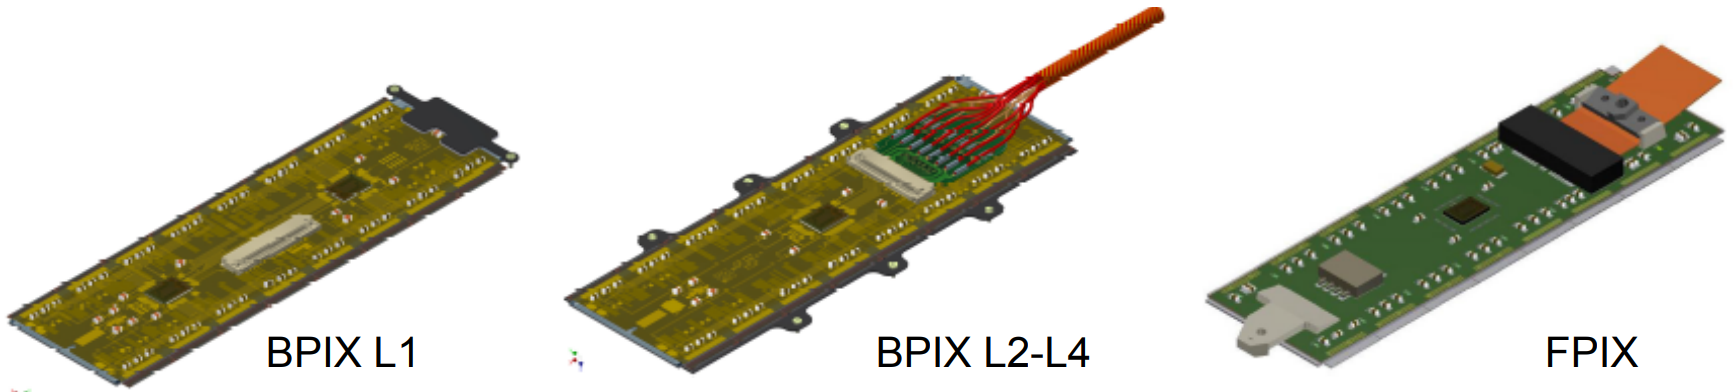
\includegraphics[scale=.2]{Chapter2/modules_drawing.png}
    \caption[Pixel detector modules]{ Drawings of the pixel detector modules for BPIX L1 (left), BPIX L2–4 (middle), and the FPIX detector (right)\cite{phase1_Pixel_Detector}.}
    \label{modules_drawing}
  \end{figure}
\end{center}


In the BPIX detector, the orientation of the sensor surface of the modules is parallel to the magnetic field. The pixels are oriented with the long side parallel to the beam line. In the FPIX detector, the modules in the outer rings are rotated by 20$^{\circ}$ in a turbine-like geometry. However, to obtain optimal resolution in both the azimuthal and radial directions for the inner ring, the modules in the inner ring are arranged in an inverted cone array tilted by 12$^{\circ}$ with respect to the beam line, combined with the 20$^{\circ}$ rotation. The sensor orientation in the FPIX detector is such that the long side of the pixel is in the radial direction \cite{phase1_Pixel_Detector}.

The sensors of the BPIX and FPIX detectors were produced by different companies in order not to depend on a single source. The concept and design were tailored to each vendor's production process, leading to two different sensor types. Both types of sensors are made of silicon and follow the n-in-n approach, with strongly n-doped (n+) pixelated implants on an n-doped silicon bulk and a p-doped back side. In a reverse-bias configuration, the n+ implants collect electrons \cite{phase1_Pixel_Detector}.\\
%%%%%%
%In the pixels, the interface between the silicon substrate and the silicon oxide carries a slight positive charge which increases by orders of magnitudes after ionizing radiation. This causes a conducting electron accumulation layer, which may short the electron-collecting electrodes. Therefore an n-side isolation is required. The technical implementation of this isolation has a large impact on the pixel cell layout and was chosen to best match the techniques offered by the two vendors.
A Photograph of four pixel cells on a BPIX sensor and schematic of two pixel cells on an FPIX sensor is shown in Fig. \ref{photo_pixel}.% In the case of the BPIX sensors, the n-side isolation was implemented through the moderated p-spray technique with a punch-through biasing grid (Fig \ref{photo_pixel} left). The FPIX sensors use open p-stops for n-side isolation. Each pixel is surrounded by an individual p-stop which has an opening on one side (Fig. \ref{photo_pixel} right) \cite{phase1_Pixel_Detector}.
\begin{center}
  \begin{figure}[ht]
    \centering
    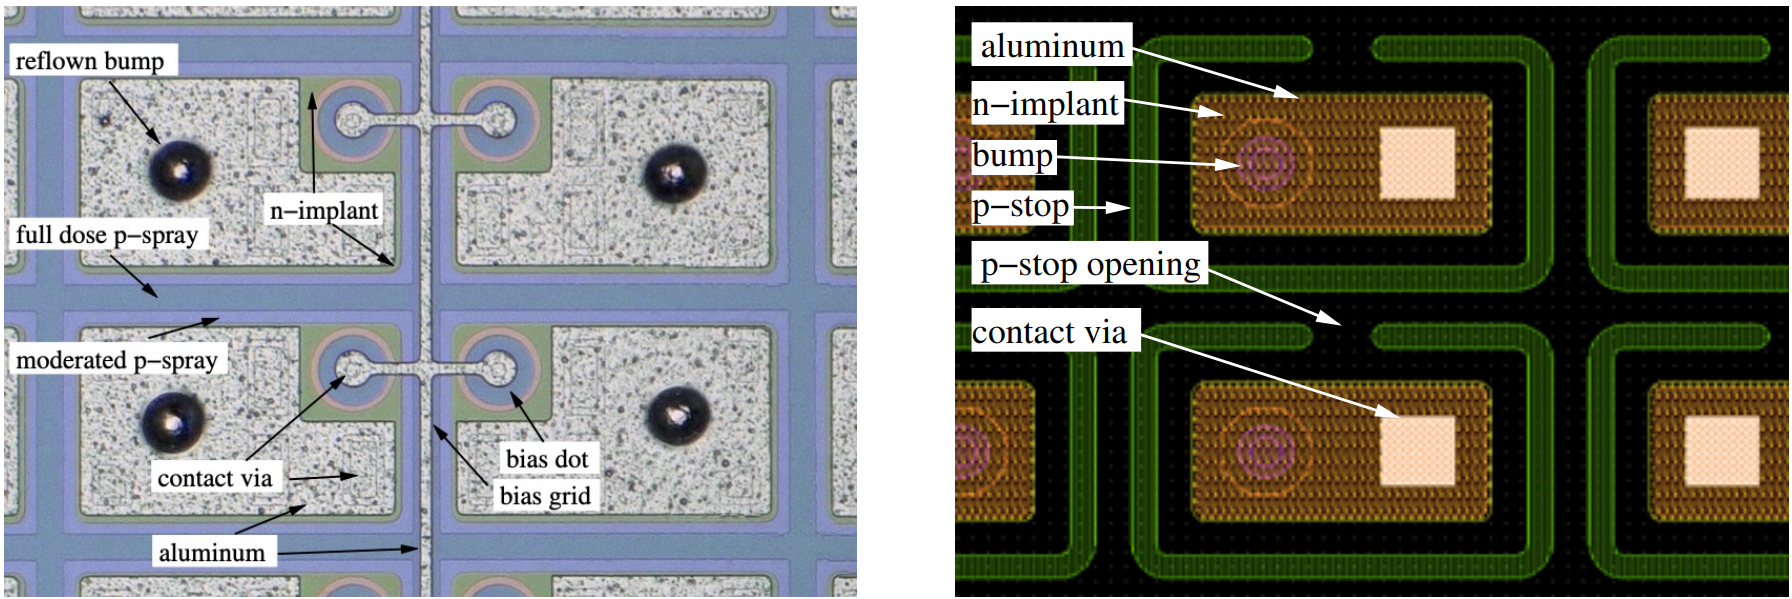
\includegraphics[scale=.2]{Chapter2/pixel_foto.png}
    \caption[Photograph of four pixels cells on a BPIX sensor and schematic of two pixel cells on an FPIX sensor]{ Photograph of four pixel cells on a BPIX -sensor (left) and schematic of two pixel cells on an FPIX sensor (right) \cite{phase1_Pixel_Detector}.}
    \label{photo_pixel}
  \end{figure}
\end{center}
%The calibration procedure includes the adjustment of phases for programming and readout signals, the determination and equalization of pixel charge thresholds, the calibration of pixel charge measurements, as well as the masking of non-working channels \cite{phase1_Pixel_Detector}.\\
%By design, the position resolution of the CMS Phase-1 pixel detector depends strongly on the charge sharing between pixels. The pixel shape of 100 $\times$ 150$\mu\text{m}^{2}$ means that in order to obtain an optimal position measurement in the azimuthal direction (the bending plane for charged particle tracks within the CMS magnet) the charge width  has to be of the order of the pixel pitch, that is 100$\mu \text{m}$. The charge width is defined as the projection on the module coordinates of the area where the charge is collected on the detector surface. In the strong magnetic field of 3.8 T provided by the CMS magnet, the Lorentz angle (LA) for the drifting electrons has a value of about 27$^{\circ}$. With the sensor thickness of 285 $\mu \text{m}$, this produces a charge width of 145 $\mu \text{m}$, which is sufficient to share the charge between at least two pixels \cite{phase1_Pixel_Detector}.\\
The most probable value of energy deposition for normally incident minimum-ionizing particles (MIPs) in a silicon sensor with a thickness of 285 $\mu \text{m}$ corresponds to approximately 21000 electrons. This charge is frequently spread over more than one pixel due to Lorentz drift and diffusion of collected electrons, leading to charge clusters. In the track reconstruction step, hit pixels are combined to form clusters from neighboring pixels. The charge measured within the cluster corresponds to the charge deposited by a single charged particle \cite{phase1_Pixel_Detector}. \\
%%%%%%%%%%%%%%%%%%%%%%%%%%% LO DE NOISE AND TRESHOLDS LO MUEVO AL SIG. CAPITULO%%%%%%%%%%%%%%%%
%The LA depends strongly on the bias voltage of the sensor and weakly on the temperature. It is also affected by the
%The lowest possible value that can be chosen for the threshold of a given pixel is an important performance parameter, since thresholds directly influence the position resolution. The strategy adopted is to adjust each ROC to its lowest possible threshold, which results in a non-uniform threshold distribution between different ROCs (with a standard deviation of about 150-200$e^{-}$). Within ROCs, pixels are trimmed to a common threshold using the available 3-bit adjustment in each pixel (resulting in an average standard deviation per ROC of about 75-100$e^{-}$). The ROCs in BPIX L1 had to be adjusted to thresholds higher than the possible minimum due to the larger cross-talk noise.\\
%The threshold and the noise are determined by recording the S-curves (as described inSec. 3.6) for a number of pixels per ROC. A subset of 81 pixels per ROC was found to be sufficient to determine the average threshold and noise values per ROC. After the initial adjustment of the pixel thresholds, periodic re-adjustments are needed. Radiation influences various parameters of the ROC, which results in threshold shifts. The pixel thresholds are closely monitored over the course of the data-taking period, and re-adjusted if necessary. During the technical stops in 2017 and at the beginning of 2018, the thresholds have been re-optimized. The BPIX L2-4 thresholds stayed roughly constant at about 1400 $e^{-}$, similarly for the FPIX detector at about 1500 $e^{-}$. For BPIX L about 2600 $e^{-}$ in 2017. After optimization in 2018, the L1 thresholds were about 2200 $e^{-}$.\\
%With these pixel thresholds the number of noise hits was very low, below 10 pixels per bunch crossing per layer, resulting in a per pixel noise hit probability of less than  $10^{-6}$. Individual pixels that showed a hit probability exceeding 0.1\% were masked during operation. The total fraction of masked pixels was less than 0.01\%
%The hit efficiency is the probability to find a cluster in a given silicon sensor that has been traversed by a charged particle <-- from 
%%%%% HEREEE
%\subsection{Strip tracker}
The rest of the tracker system surrounds the Pixel detector: the Strip tracker, as can be seen in Fig. \ref{strip_layout}. It is composed of for subsystems: the Tracker Inner Barrel (TIB) and Disks (TID), the Tracker Outer Barrel (TOB) and The Tracker EndCaps (TEC). TIB and TID are composed of four barrel layers, supplemented by three disks at each end; TOB consists of six barrel layers; Each TEC is composed of nine disks, containing up to seven concentric rings of silicon strip modules. The strip tracker has in total  15 148 silicon modules, which cover an active area of about 198$\text{m}^{2}$ and have 9.3 million strips \cite{CMS_Exp_2008}.
%Original text:
% The strip tracker is composed of for subsystems: the Tracker Inner Barrel (TIB) and Disks (TID), the Tracker Outer Barrel (TOB) and The Tracker EndCaps (TEC). Fig. \ref{strip_layout} shows an schematic cross section through the CMS trackers with the four subsystems. The TIB and TID cover $ r <\text{55 cm}$ and $|z| <\text{118 cm} 118$, and are composed of four barrel layers, supplemented by three disks at each end.  The TOB covers $r > \text{55 cm}$ and $|z| < \text{118 cm} $and consists of six barrel layers providing position measurements in $r\phi$ with a resolution of approximately 18–47$\mu \text{m}$.  The TEC cover the region 124 $< |z|$ < 282 cm. Each TEC is composed of nine disks, each containing up to seven concentric rings of silicon strip modules, yielding a range of resolutions similar to that of the TOB \cite{CMS_Exp_2008}.\\ The strip tracker has in total  15 148 silicon modules, which cover an active area of about 198$\text{m}^{2}$ and have 9.3 million strips \cite{CMS_Exp_2008}.
\begin{center}
  \begin{figure}[ht]
    \centering
    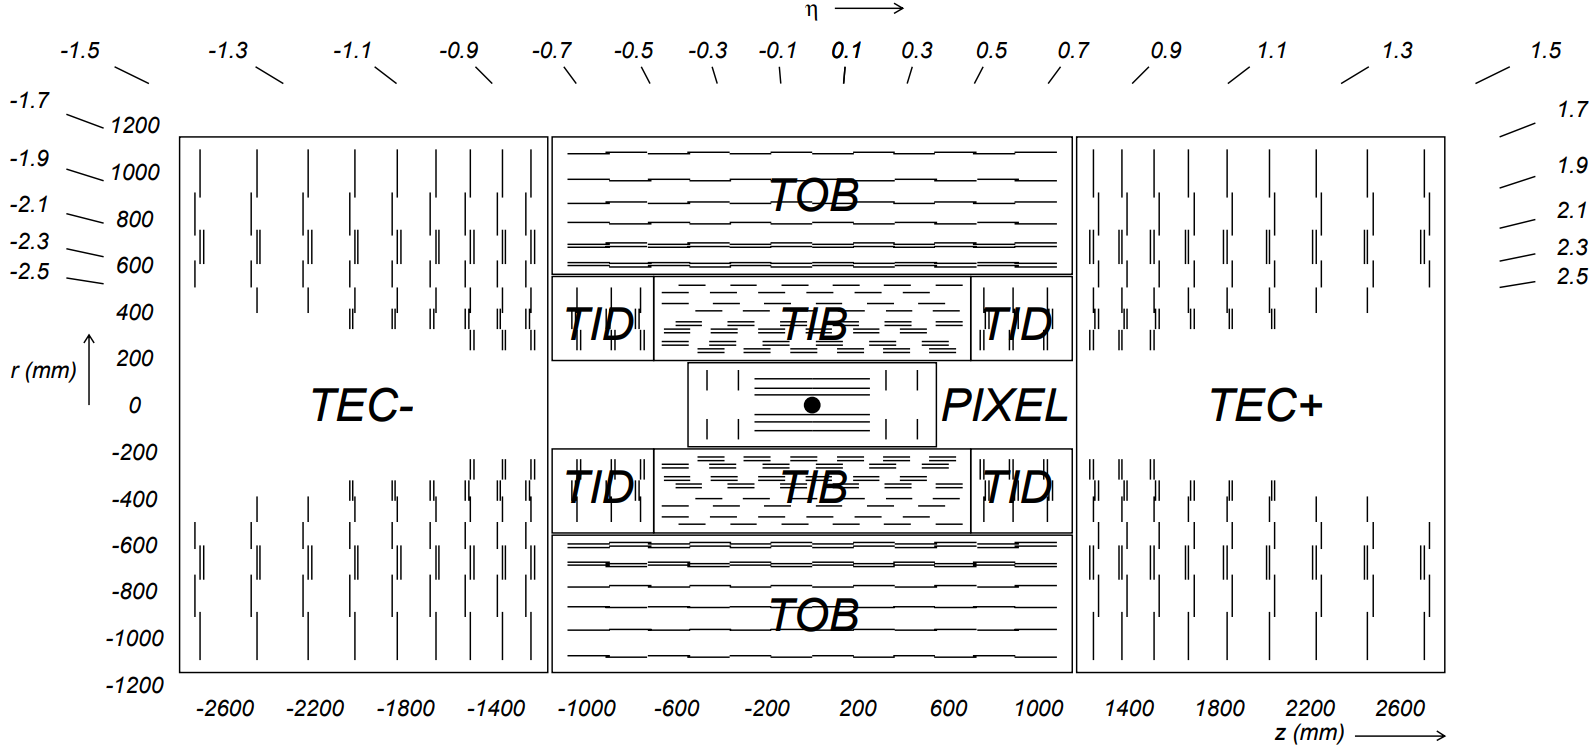
\includegraphics[scale=.23]{Chapter2/strip_layout.png}
    \caption[Schematic cross section through the CMS tracker]{Schematic cross section through the CMS tracker. Each line represents a detector module \cite{CMS_Exp_2008}. The Pixel tracker here is not the CMS Phase-1 pixel detector.}
    \label{strip_layout}
  \end{figure}
\end{center}

%\subsection{Hit/Cluster reconstruction in the Pixel detector}
The first step of the track reconstruction process is referred to as local reconstruction. It consists of the clustering of zero-suppressed signals above specified thresholds in pixel channels into hits, and then estimating the cluster positions and their uncertainties defined in a local orthogonal coordinate system $(u,v)$ in the plane of each sensor. The pixel sensor consists of 100 $\times$ 150$\mu \text{m}^{2}$ pixels with the u-axis oriented parallel to the shorter pixel edge. Offline, pixel clusters are formed from adjacent pixels, including both side-by-side and corner-by corner adjacent cells. Each cluster must have a minimum charge equivalent to 4000 electrons \cite{Track_Reco_2014}.
%Two algorithms are used to determine the position of pixel clusters. A fast algorithm, referred to as ``First-pass hit reconstruction'' ,is used during track seeding and pattern recognition, and a more precise algorithm, referred to as ``Template-based hit reconstruction'', is  based on cluster shaped and is used in the final track fit \cite{Track_Reco_2014} .\\
%1st algorithm
%The First-pass hit reconstruction consists of the following. The position of a pixel cluster along the transverse $(u)$ and longitudinal $(v)$ directions in the local orthogonal system are estimated independently with the same procedure. The cluster is projected onto the $u$-axis by summing the charge collected in pixels with the same $u$-coordinate. The result is referred to as a projected cluster. For projected clusters that are only one pixel large, the $u$-position is given by the centre of that pixel, corrected for the Lorentz drift of the collected charge in the CMS magnetic field. For larger projected clusters, the hit position is determined using the relative charge in the two pixels at each end of the projected cluster \cite{Track_Reco_2014}.\\
% For the pixel barrel, the Lorentz shift is approximately 59µm
%2nd algorithm
%The template-based hit reconstruction comes from the fact that the high level of radiation exposure of the pixel detector can affect significantly the collection of charge by the pixels during the detector’s useful life. This degrades particularly the performance of the standard hit reconstruction algorithm mentioned before.\\% In the template-based reconstruction algorithm, the observed distribution of the cluster charge is compared to expected projected distributions, called templates, to estimate the positions of hits. The templates are generated based on a large number of simulated particles traversing pixel modules, which are modelled using the detailed simulation of pixel sensors (PIXELAV). Since the PIXELAV program can describe the behaviour of irradiated sensors, new templates can be generated over the life of the detector to maintain the performance of the hit reconstruction. To allow the template-based algorithm to be applied to tracks crossing the silicon at various angles, different sets of templates are generated for several ranges of the angle between the particle trajectory and the sensor \cite{Track_Reco_2014}.\\
%The track reconstruction is done by using the hits, obtained from the local reconstruction, to obtain estimates for the momentum and position parameters of the charged particles responsible for the hits (tracks).
%NOTA: En la seccion 10.5 del paper de phase 2 pixel, menciononan cuantos electrones se porducen aprox. Algo de ionixacion minima
%10.4 tambien

%%%%%%%%%%%%%% FOLLOWING SECTIONS ARE SUMMARIZED ~ 2ND PARAGRAPH OF THIS CHAPTER%%%%%%5
%%%%\section{Electromagnetic calorimeter}
%%%%
%%%%The electromagnetic calorimeter of CMS (ECAL) is a hermetic homogeneous calorimeter made of 61 200 lead tungstate (PbWO4) crystals mounted in the central barrel part, closed by 7 324 crystals in each of the two endcaps. A preshower detector is placed in front of the endcap crystals. Avalanche photodiodes (APDs) are used as photodetectors in the barrel and vacuum phototriodes (VPTs) in the endcaps. The use of high density crystals has allowed the design of a calorimeter which is fast, has fine granularity and is radiation resistant, all important characteristics in the LHC environment \cite{CMS_Exp_2008}.\\
%%%%The barrel section (EB) has an inner radius of 129 cm. It is structured as 36 identical “supermodules,” each covering half the barrel length and corresponding to a pseudorapidity interval of 0 $< |\eta| <$ 1.479. The crystals are quasi-projective (the axes are tilted at 3$^{\circ}$ with respect to the line from the nominal vertex position) and cover 0.0174 (i.e. 1$^{\circ}$) in$ \Delta \varphi$ and $\Delta \eta$. The crystals have a front face cross-section of $\approx$22$\times$22 mm$^{2}$ and a length of 230 mm \cite{TDR_CMS}.\\
%%%%The endcaps (EE), at a distance of 314 cm from the vertex and covering a pseudorapidity range of 1.479 $< |\eta| <$ 3.0, are each structured as 2 “Dees”, consisting of semi-circular aluminium plates from which are cantilevered structural units of 5$\times$5 crystals, known as “supercrystals.” The endcap crystals, like the barrel crystals, off-point from the nominal vertex position, but are arranged in an x-y grid (i.e. not an $\eta - \varphi$ grid). They are all identical and have a front face cross section of 28.6$\times$28.6 mm2 and a length of 220 mm. A preshower device is placed in front of the crystal calorimeter over much of the endcap pseudorapidity range. The active elements of this device are 2 planes of silicon strip detectors, with a pitch of 1.9 mm, which lie behind disks of lead absorber \cite{TDR_CMS}. Fig. \ref{ECAL} shows a transverse section of the ECAL.
%%%%
%%%%
%%%%\begin{center}
%%%%  \begin{figure}[ht]
%%%%    \centering
%%%%    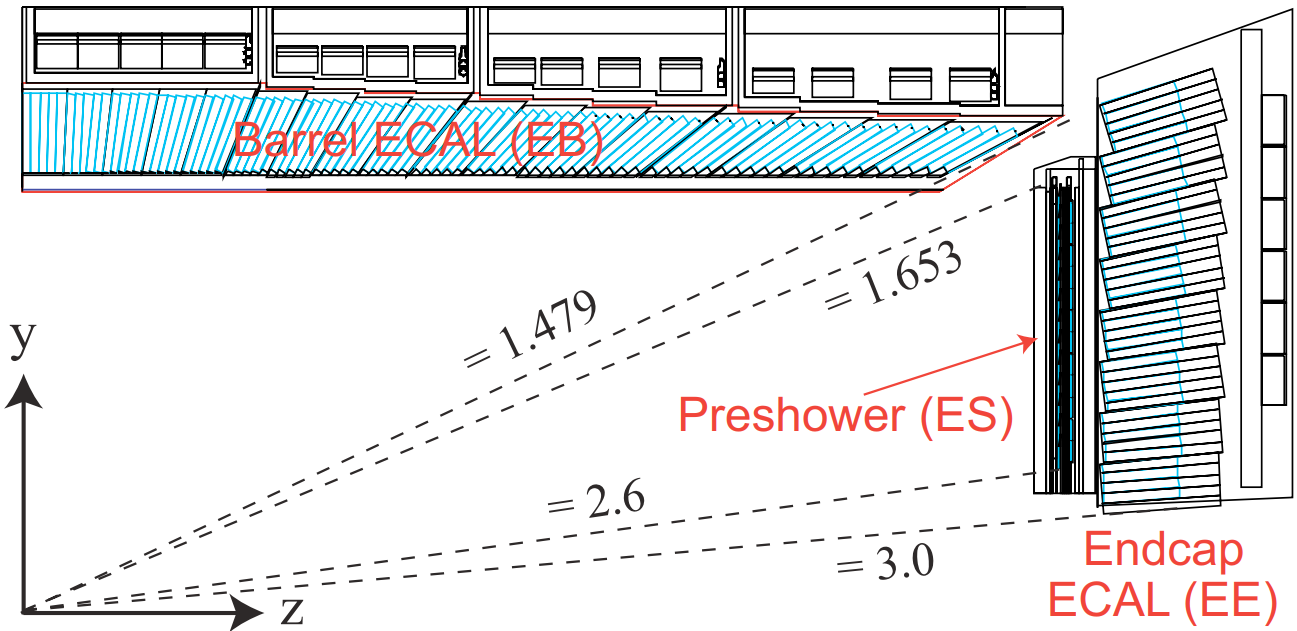
\includegraphics[scale=.25]{Chapter2/ECAL.png}
%%%%    \caption[Electromagnetic Calorimeter]{Transverse section of the  Electromagnetic calorimeter, showing geometrical configuration \cite{TDR_CMS}.}
%%%%    \label{ECAL}
%%%%  \end{figure}
%%%%\end{center}
%%%%
%%%%
%%%%\section{Hadron calorimeter}
%%%%The ECAL is surrounded by a brass/scintillator sampling hadron calorimeter (HCAL) with coverage up to $|\eta|<$3.0. The scintillation light is converted by wavelength-shifting (WLS) fibres embedded in the scintillator tiles and channeled to photodetectors via clear fibres. This light is detected by photodetectors (hybrid photodiodes, or HPDs) that can provide gain and operate in high axial magnetic fields. This central calorimetry is complemented by a tail-catcher in the barrel region (HO) ensuring that hadronic showers are sampled with nearly 11 hadronic interaction lengths. Coverage up to a pseudorapidity of 5.0 is provided by an iron/quartz-fibre calorimeter. The Cerenkov light emitted in the quartz fibres is detected by photomultipliers \cite{CMS_Exp_2008}. Fig. \ref{HCAL} shows a longitudinal view of the CMS detector showing the locations of the HCAL subsystems.\\
%%%%The Hadron Barrel (HB) is a sampling calorimeter covering the pseudorapidity range $|\eta|<$ 1.3. The HB is divided into two half-barrel sections, each half-section being inserted from either end of the barrel cryostat of the superconducting solenoid and subsequently hung from rails in the median plane. The hadron calorimeter endcaps (HE) cover a substantial portion of the rapidity range, 1.3 $< |\eta| <$ 3 (13.2\% of the solid angle), a region containing about 34\% of the particles produced in the final state. In the central pseudorapidity region, the combined stopping power of EB plus HB does not provide sufficient containment for hadron showers. To ensure adequate sampling depth for $|\eta | <$ 1.3, the hadron calorimeter is extended outside the solenoid with a tail catcher called the HO or outer calorimeter. The forward calorimeters (HF) ensure full geometric coverage for the measurement of the transverse energy in the event. The calorimeter consists of a steel absorber structure that is composed of 5 mm thick grooved plates. The detector is functionally subdivided into two longitudinal segments. Half of the fibres run over the full depth of the absorber (165 cm )while the other half starts at a depth of 22 cm from the front of the detector. An even higher forward coverage is obtained with additional dedicated calorimeters CASTOR (Centauro And Strange Object Research) and ZDC (Zero degree calorimeter) and with the TOTEM (experiment TOTal Elastic and diffractive cross section Measurement) tracking detectors \cite{CMS_Exp_2008}.
%%%%
%%%%\begin{center}
%%%%  \begin{figure}[ht]
%%%%    \centering
%%%%    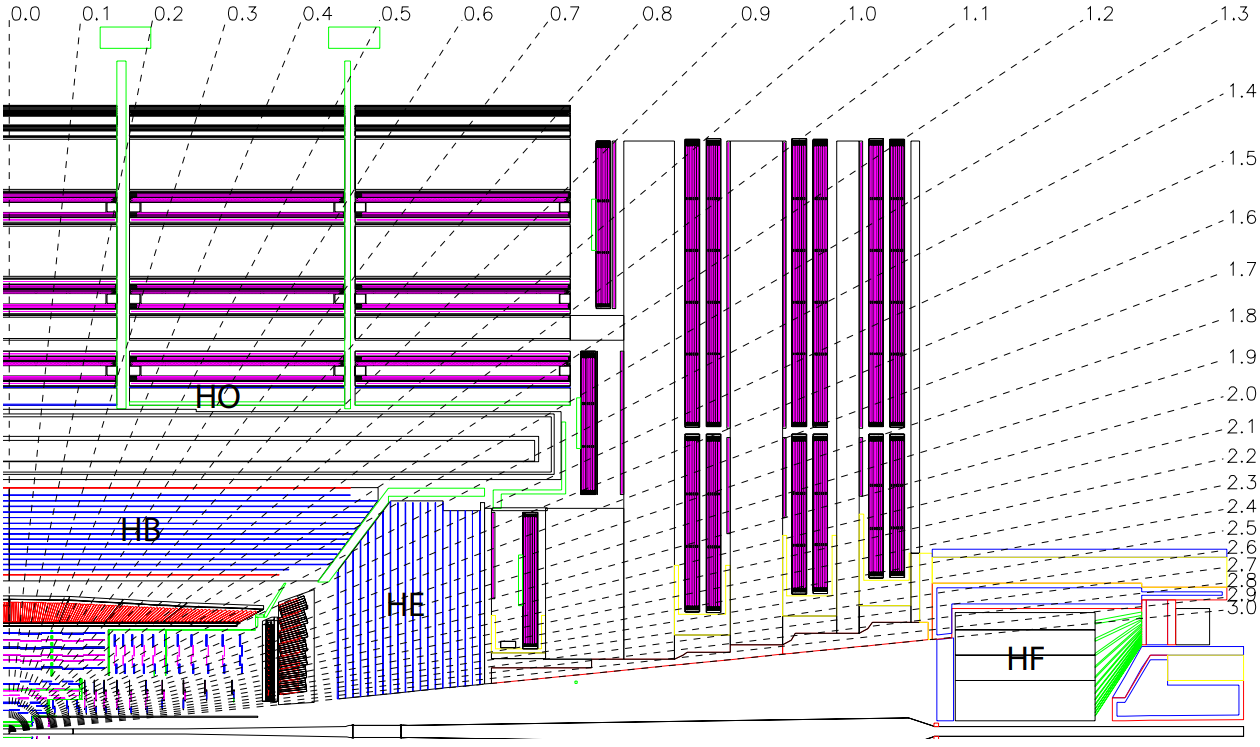
\includegraphics[scale=.3]{Chapter2/HCAL.png}
%%%%    \caption[Hadron Calorimeter]{ Longitudinal view of the CMS detector showing the locations of the hadron barrel (HB), endcap (HE), outer (HO) and forward (HF) calorimeters  \cite{CMS_Exp_2008}.}
%%%%    \label{HCAL}
%%%%  \end{figure}
%%%%\end{center}
%%%%
%%%%
%%%%\section{Muon system}
%%%%
%%%%After the HCAL and the 13-m-long, 6-m-inner-diameter, 4-T superconducting solenoid, the muons detector system is placed. The CMS muon system is designed to have the capability of reconstructing the momentum and charge of muons over the the entire kinematic range of the LHC; CMS uses 3 types of gaseous particle detectors for muon identification. Due to the shape of the solenoid magnet, the muon system was naturally driven to have a cylindrical, barrel section and 2 planar endcap regions, where are distributed three subsystems: the Barrel Drift Tube (DT), the Cathode Strip Chambers (CSC) and the Resistive Plate Chambers (RPC) \cite{CMS_Exp_2008}. A schematic diagram of the CMS detector showing the three subsystems is shown in figure \ref{Muon_detector}. \\
%%%%The barrel DT chambers cover the pseudorapidity region $|\eta| <$ 1.2 and are organized into 4 stations interspersed among the layers of the flux return plates. The first 3 stations each contain 8 chambers, in 2 groups of 4, which measure the muon coordinate in the $r- \varphi$ bending plane, and 4 chambers which provide a measurement in the $z$ direction, along the beam line. The fourth station does not contain the $z$-measuring planes \cite{CMS_Exp_2008}.\\
%%%%In the 2 endcap regions of CMS,  the muon system uses cathode  CCS. The  CSCs identify muons between $|\eta|$ values of 0.9 and 2.4. There are 4 stations of CSCs in each endcap, with chambers positioned perpendicular to the beam line and interspersed between the flux return plates. The cathode strips of each chamber run radially outward and provide a precision measurement in the $r-\varphi $ bending plane. The anode wires run approximately perpendicular to the strips and are also read out in order to provide measurements of $\eta$ and the beam-crossing time of a muon. Each 6-layer CSC provides robust pattern recognition for rejection of non-muon backgrounds and efficient matching of hits to those in other stations and to the CMS inner tracker \cite{CMS_Exp_2008}.\\
%%%%A complementary, dedicated trigger system consisting of RPC was added in both the barrel and endcap regions. The RPCs provide a fast, independent, and highly-segmented trigger with a sharp $p_{T}$ threshold over a large portion of the rapidity range  ($|eta| <$ 1.6) of the muon system. A total of 6 layers of RPCs are embedded in the barrel muon system, 2 in each of the first 2 stations, and 1 in each of the last 2 stations \cite{CMS_Exp_2008}. 
%%%%
%%%%
%%%%\begin{center}
%%%%  \begin{figure}[ht]
%%%%    \centering
%%%%    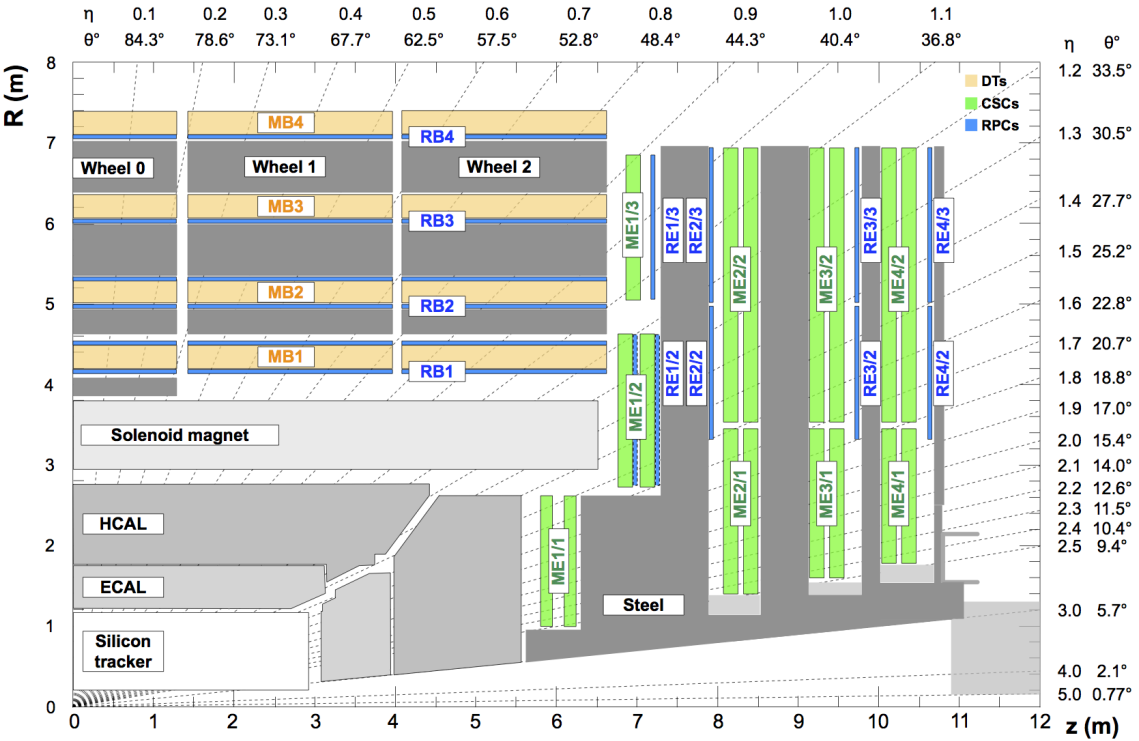
\includegraphics[scale=.3]{Chapter2/MuonDetector_Layout.png}
%%%%    \caption[Muon Detector]{ An $R-z$ cross section of a quadrant of the CMS detector with the axis parallel to the beam ($z$) running horizontally and the radius ($R$) increasing upward. The locations of the various muon stations are shown. The drift tube stations (DTs) are labeled MB (“Muon Barrel”) and the cathode strip chambers (CSCs) are labeled ME (“Muon Endcap”). Resistive plate chambers (RPCs) are mounted in both the barrel and endcaps of CMS, where they are labeled RB and RE, respectively \cite{MuonDetPerf_CMS}.}
%%%%    \label{Muon_detector}
%%%%  \end{figure}
%%%%\end{center}
%%%%

\subsection{CMS Luminometers}
Various systems are used for measuring luminosity at CMS. The Pixel Luminosity Telescope (PLT) and Fast Beam Conditions Monitor (BCM1F) are dedicated systems for luminosity measurement, while the hadronic forward calorimeter (HF) uses a dedicated readout on an existing system; these three use a separate data acquisition (DAQ) system, BRILDAQ, which operates independently of the main CMS readout \cite{pas_18}.\\
The PLT uses silicon pixel sensors arranged into 16 “telescopes”, each having three sensor planes arranged nearly parallel to the beam pipe, where the rate of “triple coincidences” is measured; a hit is observed in all three planes.\\
BCM1F consists of a total of 24 sensors mounted on the same carriage as the PLT, consisting of a total of 10 silicon sensors, 10 polycrystalline diamond (pCVD) sensors, and 4 single-crystal diamond (sCVD) sensors.\\
The HF luminosity measurement uses a dedicated readout system installed in the HF calorimeter. Only two HF rings are used for luminosity measurement, to ensure relatively uniform occupancy. Two algorithms are available: the first relies on the fraction of occupied towers (HFOC), and the second is based on the sum of the transverse energy ET (HFET).\\
In addition other methods that uses data from existing parts of the CMS detector performs a luminosity measurement using the main CMS DAQ system. One of them is the drift tube luminosity (DT) which uses the rate of muon track stubs in the muon barrel track finder. Also, the RAMSES detectors, a CERN radiation and environmental monitoring sytem, although not being designed as a luminometer does function quite well as a luminosity measurement; it uses the rate observed in the detectors (primarily photons within the energy range of 50 keV to 7 MeV).\\ Other method is the pixel cluster counting (PCC), which will be described with more detail in chapter 3.
